\documentclass[11pt]{article}
\usepackage{amsmath,array}
\usepackage{amsfonts}
\usepackage{amssymb}
\usepackage{amsthm}
\usepackage{breakcites}
\usepackage{graphicx,subcaption}
\usepackage{todonotes} %[disable]
\usepackage{cleveref}
\usepackage{tikz}
\usepackage{placeins} %FloatBarrier
\usepackage{booktabs}
\usepackage{natbib}
\usepackage{authblk}
\usepackage{url}

\usetikzlibrary{arrows,shapes,calc}

\newcommand{\abs}[1]{\left|{#1}\right|}
\newcommand{\pde}[2]{{\frac{\partial {#1}}{\partial {#2}}}}
\newcommand{\pdde}[2]{\frac{\partial^2 {#1}}{\partial {#2}^2}}
\newcommand{\de}[2]{\frac{\mathrm{d} #1}{\mathrm{d} #2}}
\newcommand{\dde}[2]{\frac{\mathrm{d}^2 {#1}}{\mathrm{d} {#2}^2}}
\newcommand{\intdef}[4]{\int\limits_{#1}^{#2} #3\, \mathrm{d}{#4}}
\newcommand{\mean}[1]{\left<{#1}\right>}
\newcommand{\cor}[2]{\mathrm{cor}\left(#1, #2\right)}


\crefname{appendix}{Appendix}{appendices}
\crefname{section}{Section}{sections}
\crefname{table}{Table}{tables}
\Crefname{table}{Table}{Tables}
\crefname{equation}{Eq.}{eqs.}
\Crefname{equation}{Equation}{Equations}
\crefname{figure}{Fig.}{figs.}
\Crefname{figure}{Figure}{Figures}
\crefname{subfigure}{Fig.}{figs.}
\Crefname{subfigure}{Figure}{figures}

\captionsetup[subfigure]{labelformat=simple}
\renewcommand{\thesubfigure}{(\alph{subfigure})}
\renewcommand{\vec}[1]{\boldsymbol{#1}}
%opening
\title{Inferring causal connectivity from pairwise recordings and optogenetics}
%\title{The need to combine optogenetics with neural recordings to estimate causal connectivity}
\author[1,2]{Mikkel Elle Lepper\o{}d}
\author[2,3,4]{Tristan St$\ddot{\text{o}}$ber}
\author[1,2]{Torkel Hafting}
\author[2,5]{Marianne Fyhn}
\author[6]{Konrad Paul Kording}
\affil[1]{Institute of Basic Medical Sciences, University of Oslo, Oslo, Norway}
\affil[2]{Centre for Integrative Neuroplasticity, University of Oslo, Oslo, Norway}
\affil[3]{Department of Informatics, University of Oslo, Oslo, Norway}
\affil[4]{Department of Computational Physiology, Simula Research Laboratory, Lysaker, Norway}
\affil[5]{Department of Bioscience, University of Oslo, Oslo, Norway}
\affil[6]{Department of Neuroscience, University of Pennsylvania, Pennsylvania, USA}
\begin{document}

 \maketitle
% suggestions for referee?
\begin{abstract} % max words 150
\noindent To study how the brain works, it is essential to identify causal interactions between neurons, usually requiring perturbations. However, when using optogenetics we typically perturb multiple cells, producing a confound - any of the stimulated neurons can have affected the target neuron. Here we show how this produces large biases, and how they can be reduced using the instrumental variable (IV) framework from econometrics. The interaction between stimulation and the absolute refractory period produces a weak, approximately random signal which can be exploited to estimate causality. When simulating integrate-and-fire neurons, we find that IV estimates connectivity better than na\"ive techniques ($R^2=0.845$ vs $R^2=0.048$). The difference is important as the estimates differ when applied to experimental data from stimulated neurons with recorded spiking activity. Our IV approach is easy to implement in the context of current experimental paradigms.

\end{abstract} 

\section{Introduction}
% The brain is infinitely confounded, thus correlations are not sufficient to draw conclusions about mechanisms and this is a hard problem in brain data.
A goal of neuroscience is to understand the mechanisms or causal chains that give rise to activity in the brain, to perception, cognition, and action. 
Complex systems such as the brain are hard to understand because of the numerous ways the contributing elements may interact internally \citep{Jonas2017}. 
Because of this, it is not sufficient to know the correlations between variables or even be able to predict them.
While observing correlations within the system is relatively easy, transitioning from observed correlations to a causal or mechanistic understanding is hard.
After all, there can be many ways that the same activities emerge from distinct causal chains \citep{drton2011global, peters2017elements}. 
Reaching a mechanistic level of understanding in the human brain is nearly impossible as it contains approximately 86 billion neurons \citep{azevedo2009equal}, each of which influences many other neurons.
Even if we could record all neurons at the same time, estimating causality and producing a mechanistic understanding would be extremely challenging.

% We use observational studies, where identifiability is questionable and causality is thus typically wrong. 
Typically, we only record from a small subset of all neurons. 
The data we obtain from such recordings, e.g. from electrophysiology or calcium imaging, is observational, which means that it does not result from randomized perturbations. 
In such cases, we can never know to which level the observed activity was caused by other observed activity, or by unobserved activity. 
The unobserved neurons are called confounders.
If mechanisms are estimated from observational data in the presence of confounders, the consequence may be large errors and incorrect conclusions \citep{angrist2008mostly}. 
Unobserved neural activity confounds estimates of causal interactions and makes it difficult to estimate underlying mechanisms.

% Set up confounding
Confounding is the big threat to causal validity \citep{UpcomingMehlerPaper} irrespective of the use of simple regression techniques or advanced functional connectivity techniques \citep{stevenson2008inferring, honey2009predicting, aitchison2017or, pfau2013robust}.  
To estimate connectivity it is first and foremost important that it stems from cause and effect, therefore we use the term causal connectivity. 
Consider an example where we want to estimate causal connectivity between two observed, but unconnected neurons, $ A $ and $ C $ (\cref{fig:intro}(a)). 
A third unobserved neuron $ B $, is driven together with $ A $ by a common input and they are thus strongly correlated.
Furthermore, $ B $ and $ C $ are connected, thus the input drives $ C $ through $ B $.
Consequently, $ A $ and $ C $ are also correlated and the regression $ C = \beta A $ will misleadingly conclude a direct interaction when causally interpreted. 
In this case, we say the regressor $ A $ is endogenous and the regression coefficient $ \beta $ estimates the magnitude of association rather than the magnitude of causation. 
Na\"ive regressions in partially observed systems will generally not reveal causality.

% Why do we not use GLM
A much used method for estimating the output of single neurons is to perform multiple regression analyses \citep{pillow2008spatio}, modeling each neuron with a generalized linear model (GLM). 
Multiple regression may be a solution to confounding problems as they support ``explaining away" background activity \citep{stevenson2008inferring}.
However, this is only a good strategy if most neurons are included in the recordings.
Furthermore, only under certain assumptions about nonlinearity or noise sources does a fully observed system become identifiable \citep{daniusis2012inferring,shimizu2006linear}.
This is rarely the case in experimental settings, especially in the mammalian brain.
Thus, brain data, will almost never satisfy the criteria needed for identifiability \citep{pearl2009causality}. 
We thus aim to develop methods that can identify causal connectivity between neuron pairs.

% Stimulation is an intervention which is needed to estimate causal interactions
To estimate causal relationships between neurons, stimulating the pre-synaptic neuron is the gold standard. 
In fact, a common definition of causality is in terms of the effect of changing one variable in the system, independently of changing other variables -- an intervention \citep{pearl2009causality}. 
If we stimulate single neurons, the ability to estimate causal relationships by regression is within reach. 
However, this is experimentally challenging and yield low cell count because it requires intracellular, juxtacellular or two-photon stimulation \citep{pinault1996novel, lerman2017two, nikolenko2007two, emiliani2015all}. 
Because gold-standard perturbations are challenging, it is necessary and highly desirable if causality could be obtained from optogenetic stimulation in combination with neural recordings of large populations of neurons \citep{boyden2005millisecond, zemelman2002selective}.

% Optogenetic stimulation is usually totally non-local, producing confounders
Interpreting the results from optogenetic stimulation in terms of causal interactions is difficult. 
In most experimental settings, optogenetic stimulation will affect many neurons simultaneously. 
Hence, the stimulus will produce a distributed pattern of activity.
This distributed pattern of stimulation produces activity which then percolates through the network of neurons. 
Thus any post-synaptic activity induced by stimulation could in principle come from any of the stimulated neurons introducing problematic confounders.

% Causal inference is a thing, if not done well you say stupid things
For insights into how we may resolve the confounding problem induced by optogenetic stimulation, we may look to other fields that have addressed the problem of endogenous regressors. 
The inference of causality from observational data is addressed in the fields of statistics \citep{pearl2009causality}, machine learning \citep{peters2017elements} and econometrics \citep{angrist2008mostly}. 

% Example
A commonly used approach towards causal inference in economics are instrumental variables. 
Let's say that we want to estimate the return $ \beta $ from education $ x $ to yearly wages $ y $ with the regression $ y = \beta x + u $. 
Here $ u $ are the factors other than education that contribute to yearly wages. 
One of the factors in $ u $ is a person's cognitive ability which may also affect education and thus the regressor $ x $  is correlated with the error term $ u $. 
This will imply that the regression estimate $ \beta $ will not estimate the magnitude of causation from education on wages, but rather, its association. 
In this case one may use the proximity to a college or university as an instrumental variable (IV) \citep{card1993using}. 
Proximity is a good instrument since it can only affect wages through schooling. 
We expect living in proximity of colleges and universities to give higher probability to attend without affecting other contributing factors to wages such as cognitive ability. 
Then, in order to attribute the causal effect of education on wages one may calculate the ratio of covariances $ \beta = cov(\mathrm{proximity},\mathrm{wages})/cov(\mathrm{proximity},\mathrm{education})$. 
This ratio corrects for the confounding factor.

% Worry is this really correct? Yes, its provable. IVs are (under the right assumptions) actually correct.
The IV technique has been used extensively in econometrics and is provable causal given three assumptions \citep{angrist2008mostly}. 
First, the instrument must be decorrelated with the error term. 
Second, the instrument must be correlated with the regressor. 
Third, there must be no direct influence of the instrument on the outcome variable, but only an influence through the regressor variable. 
The validity of these assumptions is central when using the IV approach.

% Refractory period as an IV
For an instrument to be good, it needs to be unaffected by other variables. 
In the brain, almost everything is affected by the network state. 
However, certain variables can be more or less affected. 
For example, the overall activity of the network is due to slow and strongly nonrandom dynamics. 
In contrast, the temporal pattern of when a neuron is in a refractory state may be random. 
First, if neurons are spiking according to conditional Poisson distributions, their exact timing conditioned on the network state, will be random. 
While refractoriness may not be perfectly random, the exact times of spiking are notoriously difficult to predict \citep{stevenson2008inferring} suggesting that refractoriness is sufficiently random.

% Here we
Here we show that the IV technique can be employed if one seeks to estimate the causal connectivity between neuron pairs. 
We begin by showing how confounding factors are introduced by conventional optogenetic stimulations. 
We then simulate this confounding effect in a simple network of three leaky integrate and fire (LIF) neurons. 
With this simple model we show that by using the refractory period as an IV we are able to distinguish between connected and unconnected neuron pairs. 
We compare these estimates with a na\"ive, although widely used, cross-correlation histogram (CCH) method that fails to distinguish respective pairs. 
We then turn to a simulated network of randomly recurrent connections of excitatory and inhibitory LIF neurons with distributed synaptic weights. 
With this data at hand, we first calculate the mean squared errors of the IV method and show that it is robust to different simulated network states. 
We also compare the amount and size of false positive and false negative estimates and goodness of fit on synaptic weights with pairwise assessments using CCH and logistic regression.
Finally, we tested the methods on experimental data from extracellular recordings of single unit activity from optogenetically perturbed ensembles of neurons in the hippocampus.
The observed differences between the IV and the CCH estimate, underline the importance of considering potential confounding, when estimating connections based on neural activity.

\section{Results}
\subsection{Optogenetics is not local}
Optogenetic stimulation is generally seen as a perturbation that by and large affects neurons in proximity (< 1mm) of the light source with the effect decreasing with distance. 
However, this may be an incorrect way of conceptualizing the spatial effect of stimulation as it depends on multiple factors. 
Light intensity and opsin density are important as more light and ion channels will cause a stronger effect on each cell. 
Moreover, the number of potentially stimulated neurons is critical as more neurons will have a larger impact on the overall population activity. 
Finally, physiological properties of the cells are important as light may have a stronger effect on spiking activity when the membrane potential of the cell is sufficiently close to the firing threshold. 
The induced effect of optogenetic stimulation as a function of distance should be given by a relation between the four parameters: light intensity, spatial distribution of neurons, distributions of membrane potential across neurons, and the distribution of induced photo current.

To estimate the light intensity, we calculated the spatial extent of laser light delivered by fiber-optics under plausible experimental conditions according to \citet{Aravanis2007}; see \cref{sec:method:opto}. 
This modeling of light intensity yield an approximately $ 1/r^2 $ reduction with distance $ r $ from the stimulation site \cref{fig:concept} (cyan line). 
This is explained by the surface of a 3D shell growing with $4\pi r^2$ and photons will be roughly isotropic (but see \citep{thunemann2018does}) beyond the scattering length \cref{fig:concept} (inset). 
The same number of photons has to cross each of the spheres around the stimulation location unless they are absorbed. 
As a result, the density of photons decreases rapidly with distance.

The number of illuminated neurons at a given distance will increase with distance to the stimulation site given that neurons are uniformly distributed in brain tissue \cref{fig:concept} (black line). 
In fact, it will increase by approximately $ r^2 $ with distance. 
This derives from the same surface scaling as for the 3D shell. 
Thus the number of neurons that can be activated increases rapidly with distance.

To estimate the effect of stimulation, the functionality underlying spiking activity needs to be considered. 
This can largely be characterized by the  distribution of membrane potentials across neurons. 
Surprisingly, this distribution has been observed to be symmetrically distributed and relatively flat \citep{pare1998impact,destexhe1999impact,rudolph2006use}. 
The expected response from a pulse of light that induces a charge $Q$ should be proportional to the number of affected neurons whose membrane potential sit within a $Q/C$ range of the threshold ($C$ is the capacitance). 
Given that the distribution of membrane potentials is relatively flat (the density close to the threshold is generally within an order of magnitude of the density of its mode) suggests that the spiking response to a perturbation for any neuron is roughly proportional to the induced photo current. 
The peak amplitude of the photo current relates approximately logarithmically to the light intensity \citep{wang2007high}; see \cref{sec:method:opto}. 
Assuming that opsins are evenly distributed across neurons, the induced photo current will not be proportional with light intensity - it will fall slower. 
Based on this, we calculate the overall stimulation effect to be the product of the number of neurons in a spherical slice and the peak amplitude photo current. 
This product actually increases with distance (up to the distance where absorption becomes important) \cref{fig:concept} (blue line). 
Thus, optogenetic stimulation utilizing single photon activation does not produce a localized effect.

\begin{figure}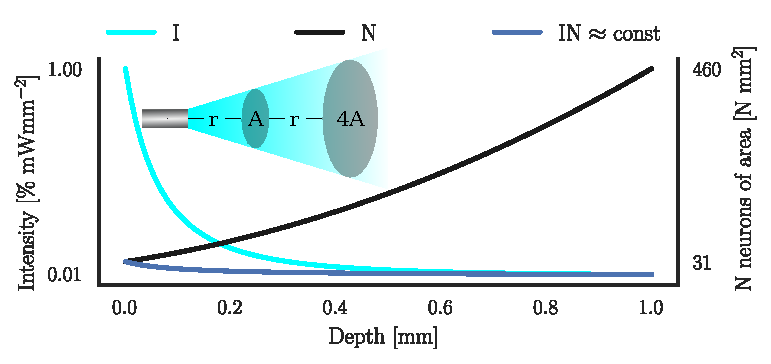
\includegraphics[scale=1]{opto-powerlaw}
\caption{{\bf Spatial extent of optogenetic stimulus}. 
Due to scattering and geometric loss the light intensity (I, cyan line) with an intensity of $10 mW/mm^2$ exiting the optogenetic fiber follows approximately an inverse square law $ r^{-2} $ where $ r $ is the distance from the fiber. 
If neurons are uniformly distributed, the number of affected neurons in a spherical slice increases by $ r^{2} $ (N, black line). 
The total photo current (sum over neurons of peak amplitude photo current in a spherical slice) thus increases with distance due to the nonlinear relation between light intensity and photo current (P, blue line) depicted as percentage of maximum.}
\label{fig:concept}
\end{figure}

\FloatBarrier
\subsection{Confounding as a problem for the estimation of causal effects}
When we stimulate many neurons at the same time, and observe a post-synaptic neuron to be active after our stimulation, it is hard to know which of the stimulated neurons produced the activity. 
To illustrate such confounding effects we simulated a network comprised of three neurons (A,B, and C) \cref{fig:intro}(a). 
The neurons receive Poisson spike trains and have Gaussian white noise added to the membrane potential. 
Neurons were also interacting, where spikes of neuron B increase the probability of firing for neuron C, but there were no other interactions.
Finally, we allowed simulated optogenetic stimulation (current pulse) to affect neurons A and B (but not C). 
We thus have a simple system for exploring questions of causality.

After running the simulation, the peri-stimulus time histogram of the stimulated neurons (\cref{fig:intro}(b)) shows the result of both the stimulation itself (suppressed for visibility) and the neuron's refractory period \cref{fig:intro}(c) (AA, BB).
Since the stimulation affects A and B simultaneously, it induces a strong correlation between A and B \cref{fig:intro}(c) (AB). 
This further generates a strong correlation between A and C, confounding the system by rendering the cross-correlation histograms (CCHs) between BC and AC both statistically significant ($ p_{\mathrm{fast}} < 0.001, p_{\mathrm{diff}} < 0.001 $; see \cref{sec:method:cch}). 
Even though the correlation peak between B and C is larger than between A and C, due to correlated spikes outside the periods with stimulation, one may imagine a situation where only A and C is measured, giving rise to a false prediction that they are connected. 
If stimulation affects multiple neurons simultaneously, there is a real confounding problem.

\begin{figure} 
\makeatletter
\renewcommand\p@subfigure{}
\makeatother
\begin{subfigure}{0.485\textwidth} 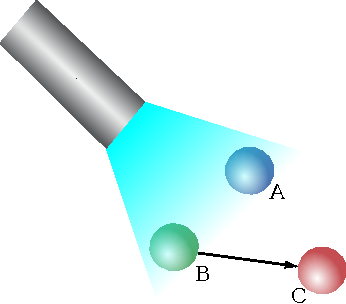
\includegraphics[scale=1]{simple}
\caption{} \label{fig:intro:1}
\end{subfigure}\hfill
\begin{subfigure}{0.485\textwidth} 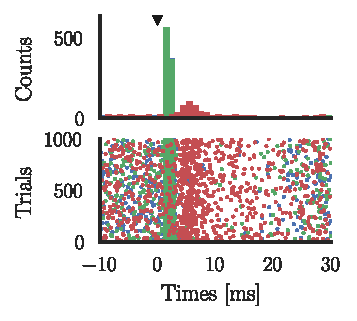
\includegraphics[scale=1]{psth_triple}
\caption{} \label{fig:intro:2}
\end{subfigure}\medskip\\
\begin{subfigure}{\textwidth}\centering 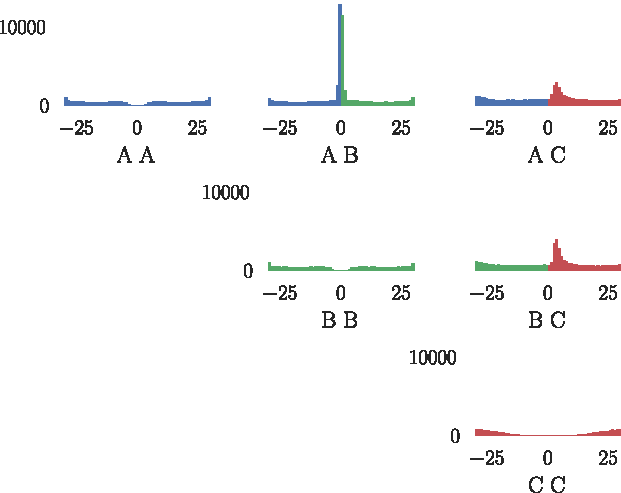
\includegraphics[scale=1]{xcorr}
\caption{} \label{fig:intro:3}
\end{subfigure}
\caption{{\bf Optogenetic stimulation induces spurious correlations}. 
A sketch of the simple network containing three neurons shows stimulation configuration with blue laser light and the connections with arrows (a). 
The neurons A and B are stimulated in 1000 trials and the corresponding peristimulus time-histogram are shown in (b) upper panel with a raster plot in the lower panel. 
Cross-correlation histograms (CCHs) are shown in (c) where horizontal and vertical axes represent time lag in ms and counts of coincident spikes in bins of 1 ms.}
\label{fig:intro}
\end{figure}

\FloatBarrier
\subsection{Instrumental variables to resolve confounding}
In order to estimate the actual influence of stimulation of a neuron on post-synaptic neurons, we need to distinguish the influence of one stimulated neuron from the influence of another stimulated neuron. 
We would thus need something that affects the stimulation effect separately between neurons. 
Arguably, refractoriness is such a variable. 
If a neuron is in its absolute refractory period, then no amount of stimulation will make it spike. 
This gives us an interesting way of inferring causality, by comparing the network state between a time when a neuron is able to spike and when the neuron is unable to spike.

Instrumental variables require the existence of a random (or sufficiently random) variable that affects the variable of interest. 
This independent influence then allows quantifying the influence of the variable of interest on the rest of the network. 
In our case, the refractory states of a neuron is in good approximation independent on small time scales (see Discussion for caveats). 
It affects the influence of stimulation on the putative pre-synaptic neuron (\cref{fig:cch_iv_triple}(a)). 
The trials where a stimuli is unable to elicit a spike due to the refractory state can then be used to identify causal effect on the putative post-synaptic neuron.

We can now investigate if the use of an instrumental variable gives a better estimate of connectivity strength than simply analyzing the lagged correlations by means of the CCH calculated with \cref{eq:ptrans} (\cref{fig:cch_iv_triple}(b, c) dashed lines). 
We use the IV estimator given by \cref{eq:wald} on the three neuron system (\cref{fig:cch_iv_triple}(b, c) solid lines). 
It converges to the correct causal conclusions that the weights $ w_{BC} = 0.2 $ and $ w_{AC} = 0 $ as opposed to the CCH method which falsely concludes that $ w_{AC} \approx 0.1 $. 
For such a simple system, it produces meaningful estimates of the causal interactions between neurons.
\tikzset{line/.style = {draw, -latex', ultra thick}}
\begin{figure}
\makeatletter
\renewcommand\p@subfigure{}
\makeatother
\begin{subfigure}{\textwidth} \centering
\begin{tikzpicture}
    \node (u) {$ S $};
    \node [above = of u] (x) {$ A/B $};
    \node [above right = of u] (y) {$ C $};
    \node [left = of x] (sr) {$ A_r/B_r $};
    \path [line] (x) -- (y);
    \path [line] (u) -- (x);
    \path [line] (u) -- (y);
    \path [line] (sr) -- (x);
\end{tikzpicture}
\caption{} \label{fig:cch_iv_triple:0}
\end{subfigure}\medskip\\
\begin{subfigure}{\textwidth} 
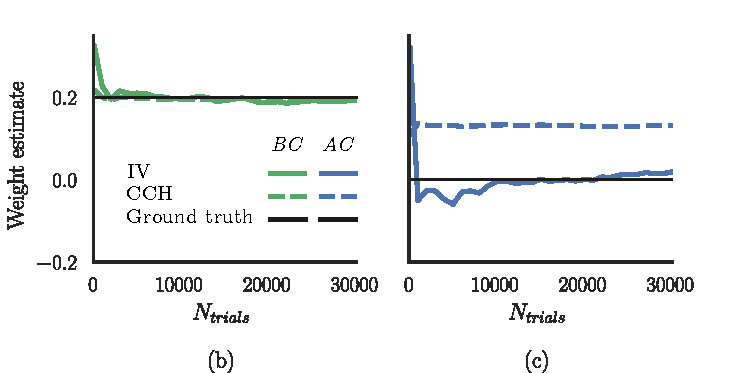
\includegraphics[scale=1]{triple}
\end{subfigure}
\caption{{\bf Instrumental variable estimation (IV) of connectivity}. 
(a) during instrumental variable estimation we use a variable that is assumed to be random (here refractoriness) which influences a variable of interest (here spiking) and to use this influence to infer the causal interaction of that variable on other variables (here spiking of A or B onto C). 
A popular estimation approach for IVs, the Wald technique, correctly estimates causal connectivity in the A, B, C system using the refractory period. 
The path diagram in (a) shows the associations between neurons $ A $, $ B $ or $ C $, the stimulation $ S $, and the IV as $ A_{r} $ or $ B_{r} $ (r for refractory).
The IV estimator calculated by \cref{eq:wald} converges to $ \hat{\beta}_{BC} \approx 0.2, \hat{\beta}_{AC} \approx 0 $ after approximately $ 5000 $ trials as seen in (b, c). 
Black line indicates ground truth and the results of the cross-correlations are showed as dotted lines. 
Note the difference between the IV estimate and CC method in (c).}
\label{fig:cch_iv_triple}
\end{figure}
\FloatBarrier

\subsection{Larger simulated networks}
Interacting neurons in a biological network exhibit inhibition and interact in many ways. 
To evaluate the IV method in a more meaningful setting we simulated a recurrent neural network consisting of 1250 randomly connected LIF neurons where 250 had inhibitory synapses. 
The network was tuned to be in an asynchronous regime; see \cref{fig:state}\labelcref{fig:CC} with log-normally distributed synaptic weights according to patch-clamp experiments \citep{Sayer1990,Mason1991}; see \cref{fig:state}\labelcref{fig:syn_dist} and \cref{tab:params} for parameters. 
Furthermore, we selected 800 excitatory neurons for stimulation and gave each neuron a random spatial distance from the simulated optogenetic stimulus. 
The stimulus intensity was then set according to \cref{eq:hill} with a maximum of 8 pA, and was constant throughout trials. 
The trial onset had a temporal Poisson distribution with period 100 ms and was further clipped between 100-150 ms. 
For weight estimates, we randomly selected among the excitatory population 100 stimulated neurons and 100 nonstimulated neurons. 

To evaluate how well the IV method estimates the weights as a function of number of trials we calculated the mean squared error of the connection weight \cref{fig:error}. 
The IV estimator's precision decreases similarly in three different settings with varying amounts of relative inhibition $ g $.
\begin{figure}
\makeatletter
\renewcommand\p@subfigure{}
\makeatother
\begin{subfigure}{\textwidth} 
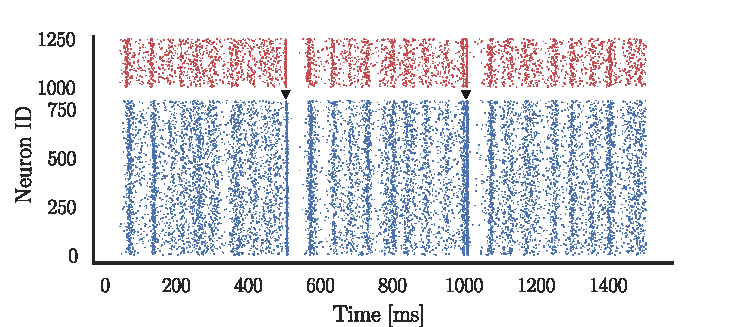
\includegraphics[scale=1]{network-raster}
\end{subfigure}\medskip

\begin{subfigure}{\textwidth} 
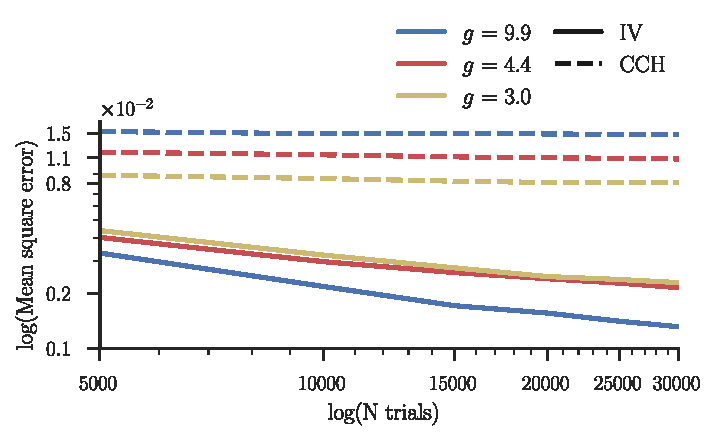
\includegraphics[scale=1]{mse}
\end{subfigure}

\caption{{\bf Mean square error (MSE) of IV and CCH based estimators in a network of two populations.} 
(a) Raster plots showing inhibitory neurons (upper panel, red) and excitatory neurons (lower panel, blue) are stimulated with varying intensity with the strongest at lower neuron number.
(b) Histogram over two stimulations, all neurons where time zero indicates stimulation onset, stimulated excitatory neurons drive inhibition which then silents the entire network.
(c, d) The IV- and CCH estimators are evaluated for the asynchronous recurrent neural network at three different amounts of relative inhibition $ g $. 
The MSE as a function of number of trials is shown in (c) on a logarithmic scale where the slopes was found to be $ -0.53, -0.48, -0.31 $ for $g = 9.9, 4.4, 3.0$ respectively. 
Finally, the MSE as a function of stimulation effect (hit rate) is shown in (d) where $hit rate = 1$ indicates that the stimulation induces a spike for each trial. \label{fig:error}}
\end{figure}

We then compared the IV estimator which exploits the refractory period, with the CCH method given by \cref{eq:ptrans} which ignores network confounding. 
We defined hit rate as the relative amount of stimulations in non-refractory states and required a minimum of 90$\%$. 
To indicate the amount of connections that are falsely attributed to a non-zero weight, we calculated the amount of false positives. 
This was given as the percentage of estimated synapses larger than $ 0.05 $ where the true weight was $ 0 $, finding $ 99.4\% $ for CCH and $ 0.2\% $ for the IV estimator; see \cref{fig:fitness}(a). 
In addition, we compared the size of the estimations at false positive instances and found that the CCH method have significantly higher median than IV (p=0, difference ($\Delta$) = 0.164, permutation resampling \citep{wassermann2006all}). 
The IV approach, while not being perfect, thus outperforms the CCH approach.

It might be that modeling refractory periods in the context of a na\"ive regression estimates connectivity equally well as the IV method. 
We thus performed a logistic regression \cref{fig:fitness}a denoted LOGIT. 
Here, we show that LOGIT performs worse than CCH illustrating the advantage of using the refractory period as an instrumental variable (p=0, $\Delta$ = 0.577, permutation resampling). 
To further evaluate the methods, we calculated false negatives as instances where the true weight is non-zero but estimated to be zero in \cref{fig:fitness}(b) shows that the CCH and IV estimators perform equally well (p=0.59, $\Delta$ = 0.017, permutation resampling), while LOGIT have no false negatives. 
Finally, we wanted to evaluate the estimated weights as a function of true weights shown in \cref{fig:fitness}(b,c) after 30000 trials. 
The IV estimator yields a good prediction ($ R^2 = 0.770 $), while the CCH method mainly estimates the strength of stimulation while true weights are poorly estimated ($ R^2 = 0.009 $). Utilizing refractory periods as an instrumental variable considerably improves the estimations.

\begin{figure}
\makeatletter
\renewcommand\p@subfigure{}
\makeatother
\begin{subfigure}{\textwidth} 
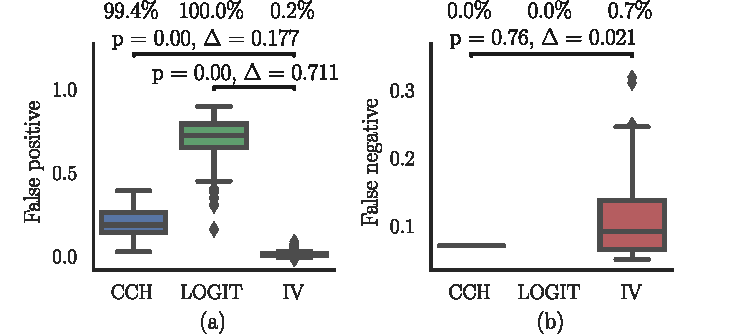
\includegraphics[scale=1]{false_estimate}
\end{subfigure}

\medskip
\begin{subfigure}{\textwidth} 
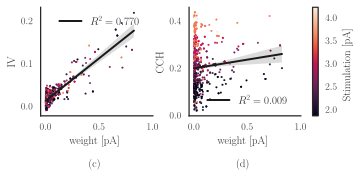
\includegraphics[scale=1]{goodness_fit}
\end{subfigure}
\caption{{\bf False estimates and goodness of fit}. 
False positives are shown in (a) for the CCH method, logistic regression (LOGIT) and the IV estimator. 
False negatives for CCH and IV are shown in (b). 
Positive estimates of weight as a function of true weight are scattered for the IV estimator in (b) and CCH in (c), color coded by the size of perturbation intensity. 
Shaded area shows the 95 \% confidence interval calculated by boot-strapping. 
Data were obtained from simulation of model 1 \cref{tab:params}.
\label{fig:fitness}}
\end{figure}
\FloatBarrier

\subsection{IV and CCH estimates from hippocampal spike recording with concurrent optogenetic stimulation}
To test the feasibility of the IV approach on \textit{in vivo} data, we compared the CCH and IV estimators on openly available extracellular single unit recordings from two mice with light-pulse stimulations of CA1 pyramidal neurons \citep{English2017}.
We investigated connections from potentially pre-synaptic units, that exhibited a significant increase in their firing rate upon stimulation, with potentially post-synaptic units that did not respond to the stimulation \citep{English2017}. 
These experiments were not optimally designed for the use of the IV method to infer causal connectivity.
Because of a low stimulation hit rate, we used an IV window of $ 7.5 $ ms, larger than the absolute refractory period of pyramidal cells, $ 4 $ ms.
This allows a proof-of-principle evaluation of the IV method on experimental data.

We want to know to what degree the IV method can be used on experimental data and if it gives different results. 
Indeed, when we apply the IV method, \cref{fig:optodata}, it seems to work robustly. 
Although we find that the results from IV are somewhat correlated with those from CCH (correlation coefficient of $0.24$), there are considerable differences between the methods. 
In many cases the confidence bounds of the two methods are truly non-overlapping, suggesting that the differences cannot only be explained by noise. 
These preliminary results illustrate that the IV approach may be applicable to address a broad range of causality estimation problems in neuroscience.  

\begin{figure}
\makeatletter
\renewcommand\p@subfigure{}
\makeatother
\begin{subfigure}{0.4\textwidth}
\includegraphics[width=1.\textwidth]{Optotrode.jpg}
%\vspace{3em}
\caption{} \label{}
\end{subfigure}\hfill
\begin{subfigure}{0.6\textwidth}
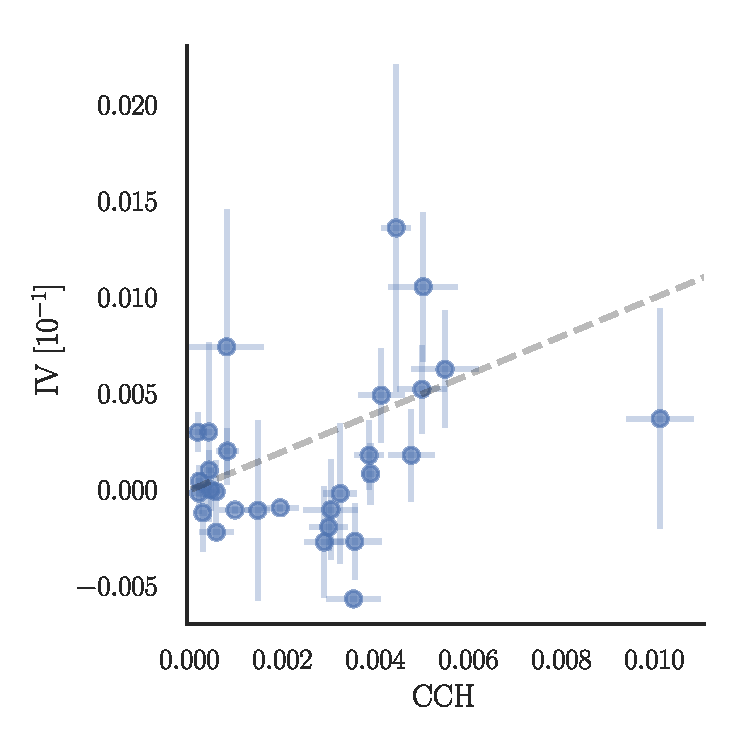
\includegraphics[width=1.\textwidth]{Optodata_comparisonIV_CCH.pdf}
\caption{} \label{}
\end{subfigure}
\caption{\textbf{IV and CCH estimates on hippocampal recording}
We compared the IV and CCH estimates of synaptic strengths on CA1 recordings with optogenetic activation of pyramidal cells \citep{English2017}.
(a) Left: schematic of the $\mu$-LED silicon probe, right: photograph of one shank tip with three illuminated $\mu$-LEDs with a scale bar at $15 \mu m$.
(b) IV and CCH estimates for connections from optogenetically activated to non-activated units that showed a significant peak in the CCH \citep{English2017}.
Dashed line represents identity. 
Error bars are $ \pm $ one standard deviation.
}
\label{fig:optodata}
 \end{figure}
\FloatBarrier
\section{Discussion}
% We have..
Here we have asked if the refractory period of neurons can be used as an instrumental variable to reverse engineer the causal flow of activity in a network of simulated neurons. 
We have found that this approach performs considerably better than the na\"ive method. 
We have found that neither na\"ive linear nor na\"ive logit models produce reliable estimates of connectivity between neuron pairs. 
The IV approach effectively reverse engineers causality by looking at the response that is missing because of refractoriness which effectively allows better estimates of causal effects. When applied to real data, we obtain robust estimates that differ from those of na\"ive estimators.

% No ground truth available, if they existed they should be random, short and intense
At the moment, we have no ground-truth data set at hand to test our technique and compare with other approaches. 
Ideally, we would have known causal effects from single-cell stimulation (e.g. from two-photon optogenetics) to establish causal effects. 
Such data should contain many randomly distributed, short and intensive stimulation trials combined with traditional optogenetics, designed in a way where refractoriness matter. 
Such a dataset, to the best of our knowledge, is currently not available and prevents us from testing how good our estimator would work on experimental data. 
Future experiments are needed to obtain reliable insights. 

% Correlated refractory periods is *the* failure mode. How to randomize them
For the refractory period to be a good instrument, it is necessary that it is not overly affected by the network activity. 
This will clearly be problematic in many cases. 
After all, network activity affects neuron activity and hence refractoriness. 
However, there are multiple scenarios where refractoriness will be a good instrument. 
For example, if we have balanced excitation and inhibition, we may expect largely independent refractory states of individual neurons. 
If a neuron biophysically implements something like conditional Poisson spiking, its refractory states will be random. 
Importantly, we may expect the phase of a neuron to be far more random than the activity of the network as a whole.

% Importance of properly designed experiments 
The randomness of refractory times is the one factor which makes or breaks the IV approach. 
Even if neurons' refractory states are strongly correlated during normal network operation, there may be ways of randomizing refractoriness. 
First, it would help to use a task and situation where neurons are as uncorrelated as possible. 
Second, we may use a set of conditioning pulses of stimulation to increase independence of refractory states. 
Giving one burst of stimulation which is strong enough to elicit multiple spikes from each neuron may effectively randomize their phases \citep{ermentrout2008reliability}.
Third, we may utilize chemical, behavioral, or molecular perturbations to randomize refractoriness. 
For example, we may be able to construct intracellular oscillators that are unaffected by neural activities. 
To the best of our knowledge, there has not been any attempts in neuroscience to produce good instrumental variables, so there may be many possibilities for improvements.

%Wald is pairwise, GLMs require multiple neurons
One popular way of estimating causal effects is fitting generalized linear models (GLMs) to simultaneously recorded neuron activities \citep{pillow2008spatio, roudi2009ising}. 
GLMs are multiple nonlinear regressions and require multiple neurons to perform well. 
In fact, if activity from all neurons were recorded, GLMs might be sufficient to estimate causal connections. 
However, complete recordings are not possible in the mammalian brain, especially not in primates, where recordings include only a very small subset of the neurons involved in the actual computation. 
When using GLMs one may accuratly estimate latency distributions and sequences of spikes from individual neurons. 
These ideas should, arguably, be merged with IV approaches. 
The main strength of the IV estimator presented here is that it only requires one pair to be recorded because we can utilize the randomness of refractory periods. 

The main problem with optogenetic stimulation, when used to infer connectivity, is its non-local property. 
This is due to the inverse relation between changes in light intensity and affected number of neurons combined with a logarithmic relation between light intensity and photocurrent \cite{wang2007high}. 
In addition, the distribution of membrane potentials across neurons is flat \citep{destexhe1999impact,rudolph2006use,pare1998impact} making neurons highly sensitive to perturbations. 
One could however, imagine situations where optogenetic activation was more local. 
If for example, the membrane potential distributions were skewed with the mode far from threshold, a very strong stimulus would be required for a neuron to elicit spikes. 
There could also be other ways of making optogenetic stimulation more local. 
For example, if one engineered opsins or brain tissue that are more light absorbent one could stimulate more locally. 
How to engineer more localized stimulation is an important problem when causally interrogating a system.

%Maybe weak stimulation will rescue us. No way, but cite Buszaki.
Very weak laser pulses in noisy networks might mainly elicit spikes in very few close-by neurons in each trial \citep{English2017}. 
However, the stimulus will still affect the membrane potential of many neurons further away, some of which will spike. 
Therefore, weak stimulation does not remove the principal problem of correlation based techniques. 
After all, the network still acts as a confounder and, if anything, the weak stimulation will reduce the statistical power of the approach. 
Lowering stimulation amplitudes does not appear to be a way of obtaining meaningful causal estimates.

%Causal inference techniques to fix experimental issues
There are many techniques for causal inference, most of which are largely unknown to the field of neuroscience, and are based on approximating randomness in a seemingly regular world. 
In many cases, one could use regression discontinuity designs in a spiking system \citep{BenPaper, imbens2008regression}. 
Moreover, one could use a difference in difference approach \citep{abadie2005semiparametric}. 
Matching approaches \citep{stuart2010matching, king2016propensity}, can be used when comparing similar network states and their evolution over time. 
In general, neuroscience is in a quest for causal interpretations, we should therefore be able to benefit considerably by utilizing techniques that are popular in the field of causal inference.

%Constructing good IVs; Multiple illuminations, designed sticky opsins
% Many trials needed here, good IV could possibly decrease this number
%We note that we obtained low errors from the IV estimator after relatively few trials when estimating weights in the neural network of 1250 neurons.\todo{how would this be in the brain with more variable synaptic properties?} 
%This amount of trials is not experimentally possible and we therefore foresee the need for improvements of the IV method. 
%It can be improved in two ways, either with algorithms that uses more of the information available, such as the exact stimulus latencies and/or the amount of spikes in each trial. 
%The other improvement could be to design experimental procedures that open for causal interpretation. 

%If we assume that the assumption of random refractory periods are violated somehow by the physiology, e.g.a very synchronized network. 
%To ameliorate one could introduce multiple light sources that is activated in a randomized fashion such that the intensity distribution is randomized. 
%This could be realized with e.g. laser holograms/filter or multiple micro LEDs. 
%This would in addition increase the amount of neurons targeted and thus give larger experimental yield. 
%Another possibility is to design opsins that have a fluctuating baseline levels randomizing membrane potential of affected neurons, however this could also lead to a chronic deficit in respective neural network and would thus shorten the time span of the experimental procedure. 
%But importantly, designing experiments so that causal inference is possible should be a major consideration for experimental design.

%We applied the IV method to openly-availabe optotrode recordings of hippocampal neurons with short, pulselike stimulations. 
%To its applicability, we apllied the IV method to an openly-availabe optotrode recording of hippocampal neurons with short, pulselike stimulations with high intensities and many repetitions. 
%In accordance with our simulation results, the analysis revealed that the IV and CCH estimator differ in their interpretation of synaptic strengths. 
%The IV and CCH estimates were weakly correlated. Several relative strong CCH estimates corresponded to small or even negative IV estimates. 
%But without ground truth data, we are not able to determine the causes of the diverging interpretations.
%Because of the low stimulation efficacy, we used an IV time window bigger than the refractory period, making the estimation susceptible to indirect paths, for example via feed-forward inhibition. 
%Other aspects artifacts For future applications of the IV approach, we recommend the use of strong, short and unchanging pulse stimulations with a high number of repetitions, randomized times and little onset artifacts. 
%To verify the IV approach \textit{in vivo}, one could use for example recently developed two-photon set-ups, which allow for simultaneous recording and stimulation of many neurons with single-cell precision \citep{packer2014simultaneous, emiliani2015all}. 
%Single-cell randomized manipulations and pairwise recordings allow for causal interrogation of synaptic connections. 
%Comparing transmission probabilities with IV estimates from recordings of potentially confounded wide-field stimulations may reveal the validity of the IV approach.


\section{Methods}
\tikzset{line/.style = {draw, -latex', thick}}
\subsection{Instrumental variable estimation}
A simple approximation of the connectivity strength between a pre-synaptic neuron $ x $ and post-synaptic neuron $ y $ can be to ignore external excitation and simply calculate the relation between the spike times in $ x $ and $ y $ with a regression model given by

\begin{equation}
y = \beta x + u.
\label{eq:regress}
\end{equation}
Here $ y $ is the dependent variable, $ x $ is the explanatory variable, $ \beta $ is the effect of $ x$ on $y $ and $ u $ is an unknown error term. 
\Cref{eq:regress} follows from the causal path diagram \citep{wright1921correlation,wright1923theory}
\begin{center}
\begin{tikzpicture}
    \node (u) {$ u $};
    \node [above = of u] (x) {$ x $};
    \node [above right = of u] (y) {$ y $};
    \path [line] (x) -- (y) node [midway, above] {$ \beta $};
    \path [line] (u) -- (y);
\end{tikzpicture}
\end{center}
Assuming that changes in spike times $ y $ are described by $ \beta x $ i.e. $ \de{y}{x} = \beta $ for spike times $ x \forall x,y \in C^1$. 
One problem with this idea is that in a confounded system, perfectly correlated neurons will give statistically indistinguishable $ \beta $. 
In the extreme case where two neurons are both made to fire every time they are stimulated, they will have the same weights according to \cref{eq:regress}. 
After all, during stimulation $ y=1 $ for both, even if only one of them drives the post-synaptic neuron. 
Another problem is if the network state affects both the probability of a neuron to fire and also the probability of post-synaptic neurons to fire. 
In this case, the network state can induce a correlation which will make the estimation highly biased. 
Arguably, the network state will, in all realistic models, have a dramatic influence on all neurons and the regression model is better described by
\begin{equation}
y = \beta x + u(x).
\end{equation}
Corresponding to the following path diagram

\begin{center}
\begin{tikzpicture}
    \node (u) {$ u $};
    \node [above = of u] (x) {$ x $};
    \node [above right = of u] (y) {$ y $};
    \path [line] (x) -- (y) node [midway, above] {$ \beta $};
    \path [line] (u) -- (x);
    \path [line] (u) -- (y);
\end{tikzpicture}
\end{center}
Here we have the relation $ \de{y}{x} = \beta + \de{u}{x} $. 
To get at causality we thus require some stimulation that only highlights the activity in $ y $ caused by $ x $, disassociating $x$ from $u$. 
However, the optogenetic stimulation is not specific to $x$ and will activate parts of the network activity $ u $. 
Let us assume that the stimulus renders only a subset of $u$ correlated with $x$, namely $u_s$ ($s$ denotes stimulated). 
To disassociate $x_s$ from $u_s$ we need something that can distinguish between different neurons that are stimulated. 
We thus require some instrument $ x_{s_r} $ which is (1) uncorrelated with the network $ u $, (2) is correlated with the regressor $ x_s $ and (3) not correlated with $ y $ \citep{angrist2008mostly}. 
We assume that the neurons are independent at small time scales and that stimulation additionally randomize membrane potential individually in neurons. 
We may thus use the fact that a neuron that has fired just before the stimulation will be in an absolute refractory state and hence have $ x_{s_r}=0 $ independently of $ u $, where the subscript $ s_r $ denotes stimulation during refractory state. 
This introduces times where the spike from one of the stimulated neurons are missing. 
Thus we may use the refractory period as an instrumental variable, as illustrated with the following path diagram

\begin{center}
\begin{tikzpicture}
    \node (u) {$ u_s $};
    \node [above = of u] (x) {$ x_s $};
    \node [above right = of u] (y) {$ y $};
    \node [left = of x] (sr) {$ x_{s_r} $};
    \path [line] (x) -- (y) node [midway, above] {$ \beta $};
    \path [line] (u) -- (x);
    \path [line] (u) -- (y);
    \path [line] (sr) -- (x);
\end{tikzpicture}
\end{center}
Here $ x_{s_r} $ represent times where the pre-synaptic neuron is refractory during stimulation. 
The true $ \beta $ is given \citep{wright1928tariff} by

\begin{equation}
\beta_{IV} = \de{y}{x_{s_r}} / \de{x}{x_{s_r}}
\end{equation}
This is then an estimator that compares the post-synaptic activity when a given neuron is non-refractory with the post-synaptic activity when it is refractory, thus removing the confounding.

Since our instrument $ x_{s_r} $ is binary we may calculate the IV (or more precisely Wald) estimator \citep{wald1940fitting} $ \beta_{IV} $ by
\begin{equation}
 \hat{\beta}_{IV} = \frac{\bar{y}_{s} - \bar{y}_{s_r}}{\bar{x}_{s} - \bar{x}_{s_r}} = \bar{y}_{s} - \bar{y}_{s_r}
 \label{eq:wald}
\end{equation}
Here $ \bar{y}_s $ is the average number of trials where successfully stimulating $ x $ resulted in a response in $ y $ and $ \bar{y}_{s_r} $ is the average number of trials where an unsuccessful stimulation of $x$ resulted in a response in $ y $. 
The successful stimulations of $x$ are denoted $x_s$ and thus $\bar{x}_s \equiv 1$. 
Conversely $x_{s_r}$ denotes unsuccessful stimulations of $x$ i.e. stimulations of $x$ during its refractory state and $\bar{x}_{s_r} \equiv 0$.

To utilize the refractory period as an IV on the simulated data we first picked out one window of $ 4 $ ms for each of the pre-synaptic and post-synaptic neuron with a latency relative to stimulation time of $ 0 $ and $ \tau_{syn} + D $ ms (see \cref{eq:syn}) respectively. 
By classifying each window for each trial whether $x$ contained a spike we obtained the two arrays $ y_s $ and $ y_{sr} $.

We found some negative values of the IV estimator which were largely suppressed by requiring a hit rate $ < 90\%$. 
Hit rates larger than $90\%$ happens mainly at strong stimulation intensity which lower statistical power in the IV or can lead to correlated refractory times. 
We hypothesize that strong stimulations can lead to synchrony induced by the stimulation \citep{ermentrout2008reliability}. 
This hypothesis was strengthened by observing that the negative values did not occur when the stimulation intensity was set to zero (data not shown). 
Furthermore, the simulated neural network introduces much response overlap due to synapses having identical synaptic time constants and transfer delays. 
This can interfere with inference since multiple neurons are affecting the same cell at the same time for each stimulation. 
However, this is less likely to occur in biological networks, which have high variability of synaptic properties and where firing patterns are sparser. 
These biological aspects would most likely work to the advantage of the IV method. 
Independence of refractoriness would be further improved, if in addition a clever stimulation routine was implemented such that the distribution of stimulation strength varies spatially from trial to trial.

\subsection{Cross correlation histogram}\label{sec:method:cch}
The statistical tests giving the probabilities $ p_{diff} $ and $ p_{fast} $ were done according to \cite{Stark2009, English2017}. 
Briefly, to test if the cross correlation histogram (CCH) peak was significant we employed two tests. 
By using the Poisson distribution with a continuity correction \citep{Stark2009} given by \cref{eq:poissoncontcor} we calculated $ p_{diff} $ by comparing the peak in positive time lag with the maximum peak in negative time lag, called $p_{causal}$ in \citet{English2017}. 
The probability $ p_{fast} $ represents the difference between CCH and it's convolution with a hollow Gaussian kernel \citep{Stark2009}. 
These two measures of significance were required to be $<0.01$ and given by
\begin{equation}
p(N|\lambda(m)) = 1 - \sum_{k=0}^{N-1}\frac{e^{-\lambda(m)}\lambda(m)^k}{k!} - \frac{e^{-\lambda(m)}\lambda(m)^N}{2N!}.
\label{eq:poissoncontcor}
\end{equation}
Here $ \lambda $ represents the counts at bin $ m $ and $ N $ is the number of bins considered. 
To estimate the connection weight between pairs we used the spike transmission probability first defined in \citet{English2017} as 
\begin{align}
\label{eq:ptrans}
p_{trans} = \frac{1}{n}\sum_{m=3ms}^{6ms} CCH(m) - \lambda_{Gauss}(m),
\end{align}
where $ n $ is the number of spikes detected in the presynaptic neuron and $\lambda_{Gauss}(m)$ is the CCH count convolved with a hollow Gaussian kernel at bin $m$.

\subsection{Logistic regression}
To utilize the refractory period without using it as an IV we estimated synaptic weights using a logistic regression. 
To do this we first picked out one window of $ 4 $ ms for each of the pre-synaptic and post-synaptic neuron with a latency relative to stimulation time of $ 0 $ and $ \tau_{syn} + D $ ms (see \cref{eq:syn} ) respectively. 
By classifying each window for each trial whether it contained a spike we obtained two binary arrays, the regressor $ x $ and the dependent variable $ y $ where we want to estimate the probability $ P(y = 1|x) $ by fitting the parameters $ \vec{\beta} $ such that
\begin{align}
y = \begin{cases}
	1 & \text{if } \beta_0 + \beta_1x + u > 0\\
    0 & \text{else}
\end{cases}
\end{align}
where $ u $ is an error term. 
Further, we used the logit link function such that the the probability giving the proxy for synaptic weight is given by
\begin{align}
p(x) = \frac{1}{1 + e^{-(\beta_0 + \beta_1x)}}
\end{align}
The model was fitted using the python package scikit-learn \citep{scikit-learn}

\subsection{Simulated network}
To simulate a recurrent network of excitatory and inhibitory neurons we used the leaky integrate and fire (LIF) model given by
\begin{equation}
	\de{V_m^i}{t} = - \frac{(V_m^i - E_L)}{\tau_m} + \frac{I_{syn}^i(t)}{C_m}.
    \label{eq:LIF}
\end{equation}
When the membrane potential $ V_m^{i} $ of neuron $ i $ reaches a threshold $ V_{th} $ an action potential is emitted and $ V_m^{i} $ reset to the leak potential $ E_{L} $ followed by an absolute refractory period $ \tau_{ref} $. 
The membrane time constant is represented by $ \tau_{m} $ and $ I_{syn}^{i}(t) $ denotes the post synaptic current (PSC) for neuron $ i $ modeled as a sum of alpha functions given by
\begin{equation}
	\label{eq:syn}
	I_{syn}^i(t) = \sum_{j=1}^C J_j \alpha(t - t_j - D),
\end{equation}
where $ t_j $ denotes an incoming spike through synapse $ j $ at delay $ D $ and $ C $ is the number of incoming synapses on neuron $ i $. 
The PSC amplitude is given by $ J_{j} $ and the alpha function is given by
\begin{align}
\tau_{syn}\alpha(t) = te^{-\frac{t}{\tau_{syn}}} H(t).
\end{align}
Here $ \tau_{syn} $ denotes the synaptic integration time constant and $ H $ is the Heaviside step function. 
All neurons were driven by an external Poisson process with rate $ rate_{p} $.

Synaptic weights were log-normally distributed such that the increase in membrane potential $ V_m^i $ due to one spike were restricted to lie between $ V_{syn} = 0.0 mV $ and $ V_{syn} = 2.0 mV $ based on experimental findings \citep{Sayer1990,Mason1991}. 
The synaptic distribution is shown in \cref{fig:state}\labelcref{fig:syn_dist} where the inhibitory PSC amplitude is given by $ J_{in} = g J_{ex} $ where $ J_{ex} $ denotes the excitatory synaptic weight.

To find suitable parameters yielding asynchronous activity we measured the population correlation coefficient given by
\begin{align}
\mean{CC}_{pop} = \mean{\mean{\frac{h_{i} - \mean{h_{i}}}{std(h_{i})}\frac{h_{j} - \mean{h_{j}}}{std(h_{j})}}}_{pop},
\end{align}
where $ h $ is the spike time histogram with binsize at $ 5ms $ for neuron $ i,j $ and $ \mean{\cdot} $ is the mean operator. 
The distribution of $ CC $ is shown in \cref{fig:cch_iv_triple} which were found by performing several parameter sweeps picking three parameter sets which mainly differed in firing rate (data not shown). 

To further evaluate the network state we calculated the coefficient of variation (CV) of the population given by
\begin{align}
\mean{CV} = \mean{\frac{std(ISI_i)}{\mean{ISI_i}}}_{pop},
\end{align}
where $ ISI $ denotes the inter-spike interval of neuron $ i $. 
We were unable to have the network showing an irregular state; see \cref{fig:state}\labelcref{fig:CV} partly to the finite synaptic integration time constant $ \tau_{syn} = 1 ms $. To verify that indeed this was due to $ \tau_{syn} $ we performed several simulations with lower $ \tau_{syn} $ obtaining $ \mean{CV}_{pop} > 1 $ (data not shown). 
It would likely be easier to achieve irregular network state if synapses were conductance based \citep{Kumar2008}. 
However, we settled with current based synapses as we were mainly interested in achieving an asynchronized state ($ \mean{CC}_{pop} < 0.01 $).
\begin{figure}
\makeatletter
\renewcommand\p@subfigure{}
\makeatother
\begin{subfigure}{0.485\textwidth} 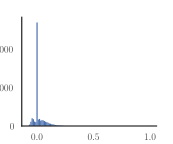
\includegraphics[scale=1]{CC}
\caption{} \label{fig:CC}
\end{subfigure}\hfill
\begin{subfigure}{0.485\textwidth} 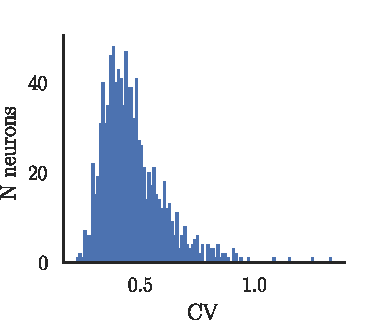
\includegraphics[scale=1]{CV}
\caption{} \label{fig:CV}
\end{subfigure}\medskip

\begin{subfigure}{\textwidth}\centering 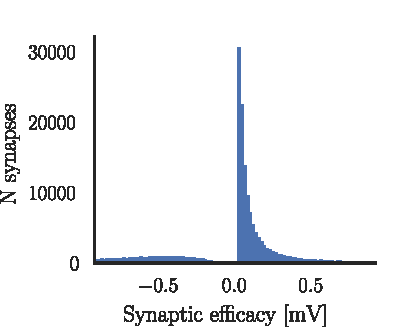
\includegraphics[scale=1]{syn_dist}
\caption{} \label{fig:syn_dist}
\end{subfigure}
\caption{Network state \label{fig:state}}
\end{figure}

\begin{table}
\centering
\begin{tabular}{lllll}
\toprule
name &    model 1 &    model 2 &    model 3 &       units \\
\midrule
$N_{neurons}$         &       1250 &        &        &             \\
$\Delta t$            &        0.1 &         &         &             \\
$N_{ex}$              &       1000 &        &        &             \\
$N_{in}$              &        250 &         &         &             \\
$eta$                 &        0.9 &         &         &             \\
$rate_{p}$            &    3694.26 &          &     &          Hz \\
$V_{reset}$           &          0 &           &           &          mV \\
$V_{m}$               &          0 &           &           &          mV \\
$E_{L}$               &          0 &           &           &          mV \\
$t_{ref}$             &          2 &           &           &          ms \\
$\tau_{m}$            &         20 &          &          &          ms \\
$V_{th}$              &         20 &          &          &          mV \\
$C_{m}$               &          1 &           &           &          pF \\
$V_{syn}$             &        0.2 &         &        &          mV \\
$g$                   &        9.9 &        4.4 &          3 &             \\
$V_{syn}^{high}$      &       2.05 &        &        &          mV \\
$V_{syn}^{low}$       &       0.05 &        &       &          mV \\
$var_{syn}$           &        0.5 &         &         &      mV$^2$ \\
$\tau_{syn}^{in}$     &          1 &           &           &          ms \\
$\tau_{syn}^{ex}$     &          1 &           &           &          ms \\
$delay$               &        1.5 &         &        &          ms \\
$eps$                 &        0.1 &        &         &             \\
$C_{ex}$              &        100 &         &         &             \\
$C_{in}$              &         25 &          &          &             \\
$J_{in}$              &    0.88727 &   0.394342 &    0.26887 &          pA \\
$J_{ex}$              &  0.0896232 &   &   &          pA \\
$J_{high}^{ex}$       &   0.918638 &    &    &          pA \\
$J_{low}^{ex}$        &  0.0224058 &   &   &          pA \\
$J_{high}^{in}$       &   0.918638 &    &   &          pA \\
$J_{low}^{in}$        &  0.0224058 &   &   &          pA \\
$time_{simulation}$   &    3685312 &        &           &         ms \\
$rate_{in}$           &    8.69 &    10.56 &     12.7 &          Hz \\
$rate_{ex}$           &    6.5 &    9.22 &    11.5 &          Hz \\
\bottomrule
\end{tabular}
\caption{\label{tab:params} Simulation parameters of three different models.}
\end{table}

\begin{table}
\centering
\begin{tabular}{lllll}
\toprule
name &    model 1 &    model 2 &    model 3 &       units \\
\midrule
$stim_{N}^{in}$       &          0 &           &           &             \\
$stim_{N}^{ex}$       &        800 &         &         &             \\
$stim_{amp}^{in}$     &          0 &           &           &          pA \\
$stim_{amp}^{ex}$     &         10 &          &          &          pA \\
$stim_{duration}$     &          2 &           &           &          ms \\
$stim_{period}$       &        100 &         &         &          ms \\
$stim_{max}^{period}$ &        150 &         &         &          ms \\

$density$             &     7514 &      &      &  Nmm$^{-3}$ \\
$S$                   &       10.3 &       &      &   mm$^{-1}$ \\
$NA$                  &       0.37 &       &       &             \\
$r$                   &        0.1 &         &         &      $\mu$m \\
$n$                   &       1.36 &        &        &             \\
$n_{Hill}$            &        0.76 &        &        &             \\
$K$                   &       0.84 &        &        &             \\
$depth$               &       0.7 &        &        &             mm\\
\bottomrule
\end{tabular}
\caption{\label{tab:params_stim} Stimulation parameters of three different models.}
\end{table}

\subsection{Calculating the mean square error}
The conditional probability of neuron $y$ firing given a spike from neuron $x$ denoted $P(y|x)$ is related to the connection strength $w_{xy}$ and the background activity. 
Since LIF neurons integrate linearly and have fixed thresholds we expect $P(y|x)$ to be proportional to the connection strength $w_{xy}$, i.e.  $P(y|x) ~ w_{xy}$. 
To calculate the mean squared errors we thus normalized $w_{xy}$ to the range $[0, max(IV_{xy})]$ or $[0, max(CCH_{xy})]$ to calculate the MSE of the IV and CCH estimators respectively by
\begin{equation*}
    MSE(w) = \frac{1}{N}\sum(\hat{w} - \bar{w})^2).
\end{equation*}We found some negative values of the IV estimator which were largely suppressed by requiring a hit rate $ < 90\%$. 
Hit rates larger than $90\%$ happens mainly at strong stimulation intensity which lower statistical power in the IV or can lead to correlated refractory times. 
We hypothesize that strong stimulations can lead to synchrony induced by the stimulation \citep{ermentrout2008reliability}. 
This hypothesis was strengthened by observing that the negative values did not occur when the stimulation intensity was set to zero (data not shown). 
Furthermore, the simulated neural network introduces much response overlap due to synapses having identical synaptic time constants and transfer delays. 
This can interfere with inference since multiple neurons are affecting the same cell at the same time for each stimulation. 
However, this is less likely to occur in biological networks, which have high variability of synaptic properties and where firing patterns are sparser. 
These biological aspects would most likely work to the advantage of the IV method. 
Independence of refractoriness would be further improved, if in addition a clever stimulation routine was implemented such that the distribution of stimulation strength varies spatially from trial to trial.
Here $\bar{w}$ is the normalized weight and $\hat{w}$ is the estimated weight.

\subsection{Calculating goodness of fit and false estimates}
The strength of the perturbations was at the maximum very large and led to many instances where the hit-rate was above 90\%. 
This represents extreme experimental conditions with very high light intensity and would yield large errors \cref{fig:error}. 
To see how the IV and CCH estimators compared we thus selected source neurons that had strictly less hit-rate than 90\%. 
This led to the maximum perturbation strength of $5pA$.

\subsubsection{Goodness of fit}
The goodness of fit was indicated by the $R^2$ value of a linear regression calculated by ordinary least squares \citep{seabold2010statsmodels} of the relation between estimated values (IV or CCH) with the true weight.

\subsubsection{False positives}
We calculated false positives from a subset $N_{sub}$ of the pairs $N$ where the true weight was $w = 0$. 
Then a false positive was defined as an estimate that were larger than $0.05$. 
The percentage of false positives was then calculated by $N_{sub}(x > 0.05) / N_{sub}$.

\subsubsection{False negatives}
We calculated false negatives from a subset $N_{sub}$ of the pairs $N$ where the true weight was $w = 0$.  
Then a false negative was defined as an estimate that had a difference from the true weight which were larger than $0.05$. 
The percentage of false negatives was then calculated by $N_{sub}(|x - w| > 0.05) / N_{sub}$.

\subsection{Perturbation intensity}\label{sec:method:opto}
In order to replicate an optogenetic experiment we modeled transmission of light through brain tissue with the Kubelka-Munk model for diffuse scattering in planar, homogeneous, ideal diffusing media \citep{Ho2017} given by
\begin{align}
T = \frac{1}{Sr + 1}.
\end{align}
Here $ T $ denotes a transmisison fraction, $ S $ is the scattering coefficient for mice \citep{Aravanis2007} and $ r $ is the distance from a light source. 
Further we combined diffusion with geometric loss assuming that absorption is negligible as in \cite{Aravanis2007} and computed the intensity as presented in \cref{fig:concept} by
\begin{align}
\label{eq:intensity}
\frac{I(r)}{I(r=0)} = \frac{\rho^2}{(Sr + 1)(r + \rho)^2}
\end{align}
where $ r $ is the distance from the optical fiber and
\begin{align}
\rho = \frac{d}{2}\sqrt{\left(\frac{n}{NA}\right)^2 - 1}.
\end{align}
Here $ d $ is the diameter of the optical fiber, $ NA $ is the numerical aperture of the optical fiber and $ n $ is the refraction index for gray matter \citep{Ho2017}; see numerical values for parameters in \cref{tab:params_stim}.

To estimate the distribution of light intensity on stimulated neurons we distributed $ 795 $ neurons uniformly in 10 spharical slices in the range $[0, 1 mm]$ which had a radius given by the cone shaped light; see \ref{fig:concept} inset.

To further estimate the peak amplitude photo current we used the Hill equation fitted by parameters found in \citet{wang2007high} given by 
\begin{equation}
    P = I_{max} \frac{I^n}{K^n + I^n}
\label{eq:hill}
\end{equation}
Here, $I_{max} = 642 pA$ is the maximum curren, $n=0.76$ is the Hill coefficient and $K = 0.84 mW/mm^2$ represents the half-maximal light sensitivity of the ChR2. 
We further used the light intensity $I$ given by \cref{eq:intensity} multiplied by an initial intensity of $10mW/mm^2$. 

Since the model neurons are not scaled to mimic ``realistic'' values in their membrane potential we set the maximum stimulation strength to $ 8 pA $ which was found suitable by investigating the percentage of successful stimulations to be $ < 100\% $. 
We then selected $ 100 $ of the excitatory neurons that were not stimulated as the ``target" population which together with the inhibitory neurons were not perturbed directly by the light stimulus.

\subsection{Application to hippocampal recordings}\label{sec:method:realdata}
We applied the IV method to CA1 recordings of two mice, downloaded from \url{https://buzsakilab.nyumc.org/datasets/McKenzieS/}.
These recordings came from silicon probes of four shanks with thirty two channels and had integrated $\mu$LEDs implanted in hippocampal region CA1.
Mice expressed channelrhodopsin-2 under the control of an excitatory neuron-specific promoter, CaMKII::ChR2 \citep{English2017}.
Each animal was recorded on several days, while mice freely behaved in their home cage.
Each recording lasted more than $3$ hours.
Spikes were then sorted by the experimenter using \todo{klustakwik??}.
During analysis, we treated each recording day independently.
During each session, sinusoidal and pulse stimulations lasting $10$ or more milliseconds were applied with different intensities.
The experimenter determined whether a unit was optogenetically stimulated by applying two criteria \citep{English2017}.
First, the number of spikes during each stimulation was noted and compared to the number of spikes in the same interval but two seconds before the stimulation.
A unit was considered optogenetically labeled, if the p-value of a Wilcoxon ranksum non-parametrical test of means was below $10^-10$.
Second, it was required that the absolute number of spikes during stimulation is on average 50\% larger compared to the number of spikes in same the interval, but two seconds before stimulation.

We considered only sessions containing pulse-stimulations.
At each shank, we grouped similar stimulation intensities.
By cross-correlating stimulation onset time with spikes, we quantified the required time for each intensity group to significantly increase the firing rate above baseline.
We used a bin-width of $3$ ms, calculated the baseline by taking the mean of the cross-correlogram for negative time lags, $-45$ to $-1.5$ ms, and applied a significance threshold of $0.01$ on the probability to obtain the observed or a higher count per bin of the poisson distribution with continuity correction \citep{abeles1982quantification}.
For each labeled neuron, those intensities were selected that caused a significant increase in firing probability within $7.5$ ms.
A labeled unit was only considered a putative pre-synaptic partner if the number of significant pulse stimulation events exceeded $2500$.
In total, connections between 17 putative pre-synaptic and 86 putative post-synaptic units were calculated.

We calculated the CCH based connection strength, $p_{trans}$, according to \citep{English2017} and section \labelcref{sec:method:cch}.
First, spiketrains of optogenetically labeled, putative pre-synaptic as well as unlabeled, putative post-synaptic units were binned with $0.4 ms$ binwidth.
The CCH has been convolved with a partially hollow gaussian kernel, with $10 ms$ standard deviation and a hollow fraction of $0.6$.
We selected a time window for $p_{fast}$ and $p_{trans}$ to be between $0.8$ and $2.8 ms$.
The reference negative time window for $p_{diff}$ was $-2$ to $0 ms$.
We further applied the same significance level of 0.01 applied to $p_{fast}$ and $p_{diff}$.

For computing the IV estimate, we used a window size of $7.5 ms$ and a fixed synaptic delay of $1 ms$.
IV and CCH estimates were separately bootstrapped with a sample size of $1000$.
For CCH estimates, we employed the additive property of the CCH function.
We divided spiketrains of a session in chunks of $100 s$, and calculated the CCH for each chunk.
We then randomly selected chunks, with replacement, to match the full length of the session.
CCH estimates were calculated on the sum of chunks.
For the IV estimates, we randomly chose stimulations with replacement to match the original number of stimulations and calculated the estimate on those samples.

\FloatBarrier
%-------------------------------------------------------------------------------
%                               Acknowledgments
%%-------------------------------------------------------------------------------
\section{Acknowledgments}
This research was partly funded by the Research Council of Norway Grant 231248 and the University of Oslo.
T.S (PhD fellow), M.F. (PI) are part of the Simula-UCSD-University of Oslo Research
and PhD training (SUURPh) program, an international collaboration in computational biology and
medicine funded by the Norwegian Ministry of Education and Research.
We thank Sam McKenzie and Daniel Fine English for sharing and explaining the optotrode data.
%-------------------------------------------------------------------------------
%                                 REFS
%-------------------------------------------------------------------------------
\pagestyle{empty}
\bibliographystyle{apalike}
{\footnotesize\linespread{1}
\bibliography{library}}
%-------------------------------------------------------------------------------
%                                 TODOS
%-------------------------------------------------------------------------------
%\newpage
%\listoftodos
\end{document}
